\documentclass{article}
\usepackage{coptreefigures}




\usepackage{tikz}
%\usepackage{pgflibraryshapes}
\usetikzlibrary{arrows,%
                decorations.pathreplacing,%
                backgrounds,positioning,%
                fit,%
                petri,%
                shapes.geometric,%
                shapes.misc,%
                spy,%
                trees,%
                calc,%
                matrix
              }



\def\xsetofvertices{1,2,...,7}

\def\setofvertexpointsRIsloped{0.25/0.5/1, 0.5/1.0/2, 0.75/1.5/3, 1.0/2.0/4,
  1.25/2.5/5, 1.5/3.0/6, 1.75/3.5/7, 2.0/4.0/8, 2.25/4.5/9,
  2.5/5.0/10, 2.75/5.5/11}  
\def\setofvertexpointsRI{0.25/0.5/1, 0.5/1.0/2, 0.75/1.5/3, 1.0/2.0/4,
  1.25/2.5/5, 1.5/3.0/6, 1.75/3.5/7, 2.0/4.0/8, 2.25/4.5/9,
  2.5/5.0/10, 2.75/5.5/11}  

\def\setofvertexpointsRII{0/0.5/1, 0/1.0/2, 0/1.5/3, 0/2.0/4,
  0/2.5/5, 0/3.0/6, 0/3.5/7, 0/4.0/8, 0/4.5/9,
  0/5.0/10, 0/5.5/11}  

\def\xsetofvertexpointsRII{0/1, 0/2, 0/3, 0/4, 0/5, 0/6,
  0/7, 0/8, 0/9, 0/10, 0/11} 

\def\xsetofvertexpointsRIII{\setofvertexpointsRI} 
\def\xxsetofvertexpointsRIII{0.25/0.5/1, 0.5/1.0/2, 0.75/1.5/3, 1.0/2.0/4,
  1.25/2.5/5, 1.5/3.0/6, 1.75/3.5/7, 2.0/4.0/8, 2.25/4.5/9,
  2.5/5.0/10, 2.75/5.5/11}  

\def\pnumtextX{%
       1/above left/15pt, 2/above/2pt, 3/above/5pt, 4/left/55pt, 5/above/5pt,%
       6/above/5pt, 7/above/5pt, 8/above/5pt, 9/above/5pt,%
       10/above/5pt, 11/above/5pt, 12/above/5pt, 13/above/5pt,%
       14/left/5pt, 15/left/5pt, 16/above/5pt, 17/below/5pt%
   }

\def\pnumtext{%
       1/left/5pt, 2/left/5pt, 3/left/5pt, 4/left/5pt, 5/left/5pt,%
       6/left/5pt, 7/left/5pt, 8/left/5pt, 9/left/5pt,%
       10/left/5pt, 11/left/5pt, 12/left/5pt, 13/left/5pt,%
       14/left/5pt, 15/left/5pt, 16/left/5pt, 17/below/5pt%
   }

   
\def\plabelsRIline{
    {(RIv11)--(RIv10)--(RIv9)--(RIv8)             /p1/8pt /blue},% 
    {(RIv10)--(RIv9)--(RIv8)--(RIv7)              /p2/4pt /red},%
    {(RIv9)--(RIv8)--(RIv7)--(RIv6)--(RIv5)--(RIv4)   /p3/6pt /red},%
    {(RIv11)--(RIv10)--(RIv9)--(RIv8)--(RIv7)--(RIv6) /p4/2pt /blue},%
    {(RIv5)--(RIv4)--(RIv3)--(RIv2)               /p5/15pt /red}%
   }


%% For plabels: \pvertices/\pnum/\sep/\pcolor/\prot/\ppos/\ppospt
\def\plabels{
    % RI
    {(RIv11)(RIv10)(RIv9)(RIv8)             /1/4pt /blue/0/above/-4pt/north west},% 
    {(RIv10)(RIv9)(RIv8)(RIv7)              /2/6pt /red/0/above/-4pt/north west},%
    {(RIv9)(RIv8)(RIv7)(RIv6)(RIv5)(RIv4)   /3/8pt /red/0/above/-4pt/north west},%
    {(RIv11)(RIv10)(RIv9)(RIv8)(RIv7)(RIv6) /4/2pt /blue/0/below/-4pt/base west},%
    {(RIv5)(RIv4)(RIv3)(RIv2)               /5/4pt /red/0/above/-6pt/north west},%
    % RII
    {(RIIv11)(RIIv10)(RIIv9)(RIIv8)%             
      /6/4pt/blue/0/left/-4pt/south west},% 
    {(RIIv10)(RIIv9)(RIIv8)(RIIv7)%
      /8/6pt /red/0/left/-4pt/south west},%
    {(RIIv9)(RIIv8)(RIIv7)(RIIv6)(RIIv5)(RIIv4)%
      /9/8pt /red/0/left/-4pt/south west},%
    {(RIIv11)(RIIv10)(RIIv9)(RIIv8)(RIIv7)(RIIv6)%
      /7/2pt /blue/0/right/-6pt/south east},%
    % RIII
    {(RIIIv11)(RIIIv10)(RIIIv9)(RIIIv8)%
      /12/4pt /blue/0/above/-6pt/north east},% 
    {(RIIIv10)(RIIIv9)(RIIIv8)(RIIIv7)%
      /13/6pt /red/0/above/0pt/north east},%
    {(RIIIv9)(RIIIv8)(RIIIv7)(RIIIv6)(RIIIv5)(RIIIv4)%
      /11/8pt /red/0/above/6pt/north east},%
    {(RIIIv11)(RIIIv10)(RIIIv9)(RIIIv8)(RIIIv7)(RIIIv6)%
      /10/2pt /blue/0/below/-4pt/base east},%
    {(RIIIv1)(RIIIv2)(RIIIv3)(RIIIv4)%
      /16/2pt /red/0/above/-8pt/north east},%
% Ri + Rj
    {(RIv2) (RIv1) (root) (RIIv1) (RIIv2) (RIIv3) (RIIv4) (RIIv5)%
      /14/6pt /green/0/left/-4pt/south west},% 
    {(RIv2) (RIv1) (root) (RIIv1) (RIIv2) (RIIv3)%
      /15/2pt/green/0/left/-4pt/south west},% 
    {(RIv1) (root) (RIIIv1) (RIIIv2)% 
      /17/8pt/green/0/below/0pt/base east}%
   }

%% HYPERGRAPH DEFS
\def\uelements{{(1,4)/a/1},%
  {(2,5)/a/2}, {(2,4)/a/3}, {(2,3)/a/4}, {(2,2)/a/5}, {(2,1)/a/6},%
  {(3,4)/a/7}, {(3,2)/a/8}, {(3,1)/a/9},%
  {(4,3)/a/10}, {(4,1)/a/11},% 
%
  {(3,-4)/c/1},%
  {(4,-5)/c/2}, {(4,-4)/c/3}, {(4,-3)/c/4}, {(4,-2)/c/5},%
  {(5,-4)/c/7},% 
  {(6,-3)/c/10}, {(4,-1)/c/6}, {(4,0)/c/9},% 
  {(5,-1)/c/8}, {(5,0)/c/11},%
%
  {(6,4)/b/1}, {(6,1)/b/11},%
  {(7,5)/b/2}, {(7,4)/b/3}, {(7,3)/b/4}, {(7,2)/b/5}, {(7,1)/b/6},%
  {(8,4)/b/7}, {(8,2)/b/8}, {(8,1)/b/9},%
  {(9,3)/b/10},% 
%
  {(5,1)/r/0}%
}

\def\slabels{%  \svertices/\sname/\sep/\scolor/\srot/\spos/\spospt
  {(a1)(a2)(a3)(a4)             /1/4pt /blue/4/above left/10pt},% 
  {(a2)(a3)(a4)(a7)             /2/4pt /red/-4/above right/10pt},% 
  {(a1)(a2)(a3)(a4)(a7) (a10)   /4/8pt /blue/2/above right/35pt},% 
  {(a3)(a4)(a7) (a10)(a5)(a8)   /3/4pt /red/-8/below right/18pt},% 
  {(a5)(a8)(a6)(a9)             /5/8pt /red/0/below left/0pt},% 
%
  {(b1)(b2)(b3)(b4)             /6/4pt /blue/4/above left/10pt},% 
  {(b2)(b3)(b4)(b7)             /8/4pt /red/-4/above right/10pt},% 
  {(b1)(b2)(b3)(b4)(b7) (b10)   /7/8pt /blue/2/above right/35pt},% 
  {(b3)(b4)(b7) (b10)(b5)(b8)   /9/4pt /red/-8/below right/20pt},% 
%
  {(c1)(c2)(c3)(c4)             /12/4pt /blue/4/below left/8pt},% 
  {(c2)(c3)(c4)(c7)             /13/4pt /red/-4/below right/10pt},% 
  {(c1)(c2)(c3)(c4)(c7) (c10)   /10/8pt /blue/2/below right/35pt},% 
  {(c3)(c4)(c7) (c10)(c5)(c8)   /11/4pt /red/-40/above right/7pt},% 
  {(c9)(c11)(c6)(c8)            /16/8pt /blue/0/below/-6pt},% 
%
  {(c9)(c11)(a11)(r0)           /17/4pt /green/10/below/-8pt},%
  {(a9)(a11)(r0)(b11)(b6)(b9)   /15/4pt /green/6/right/14pt},%
  {(a9)(a11)(r0)(b11)(b6)(b9)(b5)(b8)  /14/6pt /green/8/above right/12pt}%,%
}




\def\ksubstartpl{%
  $T$:\\

}%








\begin{document}


\begin{figure}[htb]
  \centering

%  \ksubstartpl
  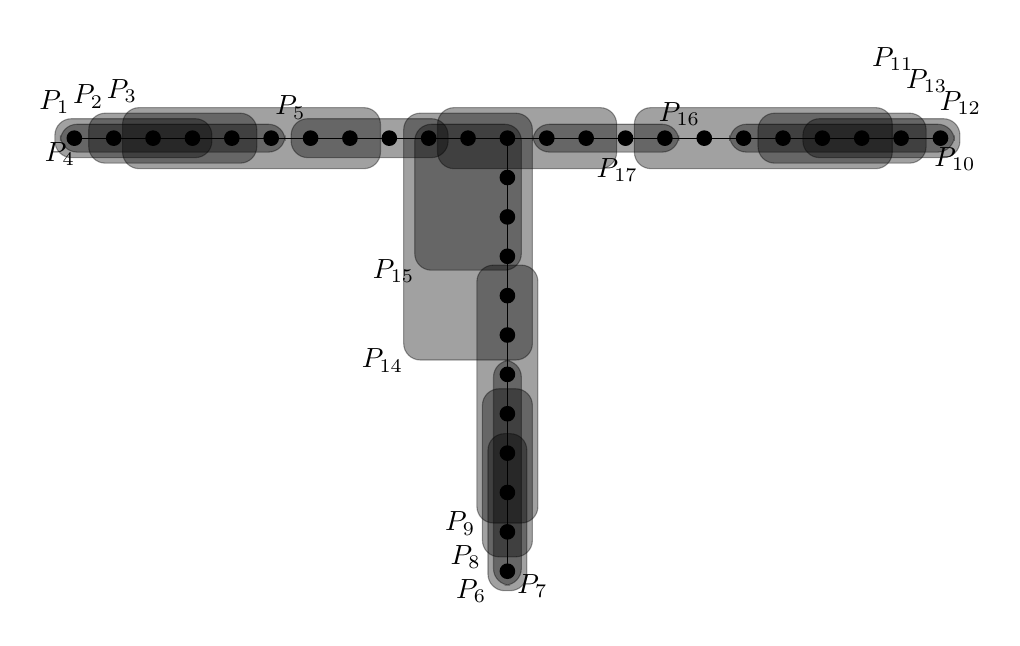
\begin{tikzpicture}[every node/.style={circle,inner
      sep=2pt,fill}]% =gray!80}] %

    %% DRAW TREE
    \draw (0,0) node (root) {}%
      \foreach \x/\y/\n in \setofvertexpointsRI {%
        -- (-\y,0) node (RIv\n) {}%{$a_{\y}$}
%        -- (-\x,-\y) node (RIv\n) {}%{$a_{\y}$}   %%% SLOPED
      }% 
    ;% 

    \draw (0,0)%
      \foreach \x/\y/\n in \setofvertexpointsRII {%
        -- (\x,-\y) node (RIIv\n) {}%{$b_{\y}$}
      }% 
    ;% 

    \draw (0,0)% RIII is a mirror image of RI
      \foreach \x/\y/\n in \setofvertexpointsRI {%
        -- (\y,0) node (RIIIv\n) {}%{$c_{\y}$}
%        -- (\x,-\y) node (RIIIv\n) {}%{$c_{\y}$}  %%% SLOPED
      }% 
    ;% 

%    \draw (root) node[fill=none, below left=2pt] {$r$};
   


    %% DRAW PATH LABELS
    \begin{pgfonlayer}{background}
      % \svertices/\sname/\sep/\scolor/\srot
     \foreach \pvertices/\pnum/\sep/\pcolor/\prot in \plabels {%      
        \node[rectangle, rounded corners=6pt, rotate fit=\prot,%
            inner sep=\sep, draw, opacity=0.37, draw,% 
            fit = \pvertices] (p\pnum) {}; %
     }
   \end{pgfonlayer}


   \foreach%
    \pvertices/\pnum/\sep/\pcolor/\prot/\ppos/\ppospt/\pposanch in%
    \plabels {% 
     \draw (p\pnum)%
       node[fill=none, \ppos=\ppospt of p\pnum.\pposanch]%
        {$P_{\pnum}$};% 
   }


  \end{tikzpicture}










  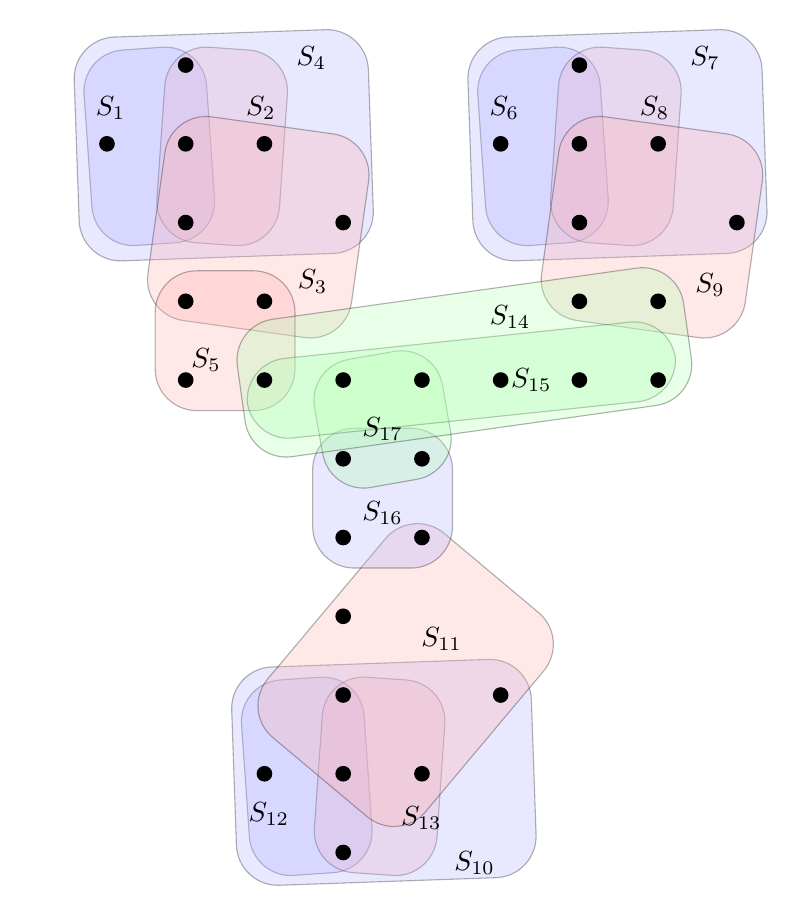
\begin{tikzpicture}[every node/.style={circle,inner
      sep=2pt}]% =gray!80}] %

  
    \draw (0,0) %
      \foreach \xy/\ray/\vnum in \uelements {%
        \xy node[fill] (\ray\vnum){}%\ray\vnum}%
      }% 
    ;% 

%     \draw (0,0)%
%       \foreach \x/\y/\n in \setofvertexpointsRII {%
%         -- (\x,-\y) node (RIIv\n) {}%{$b_{\y}$}
%       }% 
%     ;% 


    \begin{pgfonlayer}{background}

     \foreach \svertices/\sname/\sep/\scolor/\srot in \slabels {%      
        \node[rectangle, rounded corners=15pt, rotate fit=\srot,%
            inner sep=\sep, fill=\scolor!30, opacity=0.3, draw,% 
            fit = \svertices] (s\sname) {}; %
     }    
     \end{pgfonlayer}

  \foreach \X/\sname/\X/\X/\X/\spos/\spospt in \slabels {%      
    \draw (s\sname) node[\spos=\spospt] {$S_{\sname}$};
  }



  \end{tikzpicture}
  


  \caption{$k$-subdivided star tree path labeling example.}
  \label{fig:ksubstartpl}
\end{figure}



\end{document}
